
%\newpage
%\thispagestyle{frontstyle}


\chapter*{About the Author}
\addstarredchapter{About the Author}



\includegraphics[width=0.15\textwidth]{empty.pdf}\par\vspace{0.7cm}
 

\begin{wrapfigure}[14]{l}{4.2cm}
  \vspace{-12pt}
  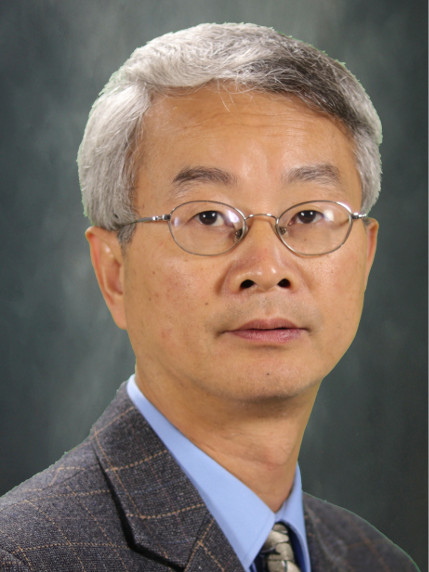
\includegraphics[width=4cm]{du_pic.jpg}
\end{wrapfigure}
\noindent \textbf{Wenliang (Kevin) Du, PhD,} received his bachelor's degree from the University 
of Science and Technology of China in 1993. After getting a Master's degree from 
Florida International University, he attended Purdue University from 
1996 to 2001, and received his PhD degree in computer science. 
He became an assistant professor at Syracuse University after the graduation. 
He is currently a full professor in the
Department of Electrical Engineering and Computer Science.


Professor Du has taught courses in cybersecurity at both undergraduate 
and graduate levels since 2001. As a firm believer of ``learning by doing'', 
he has developed over 30 hands-on labs called SEED labs, so students can 
gain first-hand experiences on security attacks, countermeasures, and 
fundamental security principles. These labs are now widely known;
more than 1000 universities, colleges, and high schools worldwide 
are using or have used these labs. 
In 2010,  the SEED project was highlighted by the National Science Foundation 
in a report sent to the Congress. The report,  titled ``New Challenges, 
New Strategies: Building Excellence in Undergraduate STEM Education (Page 16)'', 
highlights ``17 projects that represent cutting-edge
creativity in undergraduate STEM classes nationwide''. Due to the impact of the 
SEED labs, he was given the ``2017 Academic Leadership'' award from the 
\textit{21st Colloquium for Information System Security Education}. 
In 2019, Syracuse University awarded him the Meredith Professorship 
for Teaching Excellence.


Professor Du works in the area of computer and network security, with specific interests
in system security. He has published over 100 technical papers. As of April 2019, 
his research work has been cited for over 14,100 times~(based on Google Scholar). 
He is a recipient of the ACM CCS Test-of-Time Award in 2013 due to the impact of 
one of his papers published in 2003. His current research focuses on
mobile system security, aiming at 
developing novel mechanisms at the operating system and hardware levels
to enhance the security of smartphones and mobile devices. 
He also conducts research in
security education, with a focus on developing innovative 
systems that can be used for experiential learning
in cybersecurity. 
